\Annex{implémentation du \textit{clustering} interactif}
\label{annex:C-ANNEXE-IMPLEMENTATIONS}

	% INTRODUCTION.
	Au cours de ce doctorat, nous avons réalisé une implémentation en Python de notre \textit{clustering interactif}.
	Celle-ci est répartie en trois librairies :
	\begin{enumerate}
		% cognitivefactory-interactive-clustering
		\item \texttt{cognitivefactory-interactive-clustering} (\cite{schild:2022:cognitivefactory-interactiveclustering}), regroupant les gestions de données, la gestion des contraintes, les algorithmes de \textit{clustering} sous contraintes et les algorithmes d'échantillonnage implémentés ;
		% cognitivefactory-features-maximization-metric
		\item \texttt{cognitivefactory-features-maximization-metric} (\cite{schild:2023:cognitivefactory-featuresmaximizationmetric}), disposant d'une méthode de sélection des patterns linguistiques pertinents (composantes principales) d'un jeu de données, utilisée pour l'analyse de pertinence d'un résultat de \textit{clustering} ;
		% cognitivefactory-interactive-clustering-gui
		\item \texttt{cognitivefactory-interactive-clustering-gui} (\cite{schild-etal:2022:cognitivefactory-interactiveclusteringgui}), encapsulant les algorithmes précédents et intégrant la logique de la méthode dans une application web.
	\end{enumerate}
	
	Dans cette annexe, nous allons détailler ces implémentations, leurs fonctionnalités et certains des choix de mises en oeuvres.


	% TABLE DES MATIÈRES DE L'ANNEXE.
	\minitoc
	
	\todo[inline]{table de nomenclatures dans l'introduction de cette partie}
	
	
	%%%%%--------------------------------------------------------------------
	%%%%% Section C.1: Implémentation de la librairie \texttt{cognitivefactory-interactive-clustering}
	%%%%%--------------------------------------------------------------------
	%\newpage
	\section[
		\texttt{cognitivefactory-interactive-clustering}
	]{
		Implémentation de la librairie \\ \texttt{cognitivefactory-interactive-clustering}
	}
\label{annex:C.1-DESCRIPTION-IMPLEMENTATION-INTERACTIVE-CLUSTERING}
	
	% Généralités.
	La librairie \texttt{cognitivefactory-interactive-clustering} \footnote{
		\url{https://pypi.org/project/cognitivefactory-interactive-clustering/}
	} (\cite{schild:2022:cognitivefactory-interactiveclustering}) a été implémentée au cours de ce doctorat dans le but de mettre à disposition un ensemble d'algorithmes nécessaires à l'utilisation de notre méthodologie de \texttt{Clustering Interactif}.
	Cette librairie comporte plusieurs fonctionnalités :
	\begin{itemize}
		\item la gestion des données avec leurs prétraitements et leur vectorisation (cf. \textsc{Section~\ref{annex:C.1.1-DESCRIPTION-IMPLEMENTATION-INTERACTIVE-CLUSTERING-GESTION-DES-DONNEES}}) ;
		\item la gestion des contraintes avec le calcul des propriétés de transitivité et la détection des conflits (cf. \textsc{Section~\ref{annex:C.1.2-DESCRIPTION-IMPLEMENTATION-INTERACTIVE-CLUSTERING-GESTION-DES-CONTRAINTES}}) ;
		\item l'exécution d'algorithmes de \textit{clustering} sous contraintes pour proposer une segmentation des données (cf. \textsc{Section~\ref{annex:C.1.3-DESCRIPTION-IMPLEMENTATION-INTERACTIVE-CLUSTERING-ALGORITHMES-CLUSTERING-SOUS-CONTRAINTES}}) ;
		\item l'exécution d'algorithmes d'échantillonnage pour sélectionner les prochaines contraintes à annoter (cf. \textsc{Section~\ref{annex:C.1.4-DESCRIPTION-IMPLEMENTATION-INTERACTIVE-CLUSTERING-ALGORITHMES-ECHANTILLONNAGE-DE-CONTRAINTES}}).
	\end{itemize}
	
	Nous présentons succinctement cette librairie avec certains choix d'implémentation.
	
	% Information : comme y accéder.
	\begin{leftBarInformation}
		La documentation technique de cette librairie est accessible par le lien suivant : \url{https://cognitivefactory.github.io/interactive-clustering/}.
	\end{leftBarInformation}
	
	% Exemple.
	Pour les sections suivantes, nous suivrons l'exemple suivant (cf. \textsc{Code~\ref{code:C.1-DESCRIPTION-IMPLEMENTATION-INTERACTIVE-CLUSTERING-DATA}}) pour présenter nos implémentations.
	
	\begin{lstlisting}[
		language=Python,
		caption={Jeu exemple pour présenter notre implémentation du \texttt{Clustering Interactif}.},
		label={code:C.1-DESCRIPTION-IMPLEMENTATION-INTERACTIVE-CLUSTERING-DATA},
	]
# Définir les données.
dict_of_texts = {
	"0": "Comment signaler un vol de carte bancaire ?",
	"1": "J'ai égaré ma carte bancaire, que faire ?",
	"2": "J'ai perdu ma carte de paiement",
	"3": "Le distributeur a avalé ma carte !",
	"4": "En retirant de l'argent, le GAB a gardé ma carte...",
	"5": "Le distributeur ne m'a pas rendu ma carte bleue.",
	# ...
	"N": "Pourquoi le sans contact ne fonctionne pas ?",
}
	\end{lstlisting}
	
	
	%%%
	%%% Subsection C.1.1: Gestion des données.
	%%%
	\subsection{Gestion des données}
	\label{annex:C.1.1-DESCRIPTION-IMPLEMENTATION-INTERACTIVE-CLUSTERING-GESTION-DES-DONNEES}
	
	% cognitivefactory.interactive-clustering.utils
	Tout d'abord, en ce qui concerne la \textbf{manipulation de données}, nous utilisons le module \texttt{utils} de la librairie \texttt{cognitivefactory-interactive-clustering}.
	Les données sont stockées dans un dictionnaire \texttt{Python} afin de tracer les manipulations à l'aide d'une clé servant d'identifiant de la donnée.
	
	% cognitivefactory.interactive-clustering.utils.preprocessing : Implémentation.
	Nous avons d'une part la partie \texttt{utils.preprocessing} \footnote{
		\url{https://cognitivefactory.github.io/interactive-clustering/reference/cognitivefactory/interactive_clustering/utils/preprocessing/}
	} qui permet de normaliser les données.
	Par défaut :
	\begin{itemize}
		\item[\(\bullet\)] le texte est passé en \textit{minuscule} (de \textguillemets{\texttt{Bonjour}} à \textguillemets{\texttt{bonjour}}),
		\item[\(\bullet\)] la \textit{ponctuation} est supprimée \textguillemets{\texttt{c'est-à-dire ?!}} à \textguillemets{\texttt{c est a dire}}), %(\texttt{.}, \texttt{,}, \texttt{;}, \texttt{:}, \texttt{!}, \texttt{¡}, \texttt{?}, \texttt{¿}, \texttt{…}, \texttt{•}, \texttt{(}, \texttt{)}, \texttt{\{}, \texttt{\}}, \texttt{[}, \texttt{]}, \texttt{\textguillemets{}, \texttt{}}, \texttt{^}, \texttt{\`}, \texttt{'}, \texttt{"}, \texttt{\\}, \texttt{/}, \texttt{|}, \texttt{-}, \texttt{\_}, \texttt{#}, \texttt{\&}, \texttt{\~}, \texttt{\@}),
		\item[\(\bullet\)] les \textit{accents} sont enlevés (de \textguillemets{\texttt{crédit}} à \textguillemets{\texttt{credit}}),
		\item[\(\bullet\)] et les multiples \textit{espaces blancs} sont convertis en un unique espace simple (de \textguillemets{\texttt{au~~~~revoir}} à \textguillemets{\texttt{au revoir}}).
	\end{itemize}
	
	Si besoin, trois options "avancées" sont disponibles pour réaliser des prétraitements plus destructifs :
	\begin{itemize}
		\item[\(\bullet\)] la suppression des mots vides (\textit{stopwords}, \cite{nothman-etal:2018:stop-word-lists}),
		\item[\(\bullet\)] la conversion des mots vers leur forme racine (\textit{lemmatisation}, \cite{manning-schutze:2000:foundations-statistical-natural}),
		\item[\(\bullet\)] et la suppression des mots en fonction de leur profondeur dans l'arbre de dépendances syntaxiques (\cite{nivre:2006:inductive-dependency-parsing}).
	\end{itemize}
	
	% cognitivefactory.interactive-clustering.utils.preprocessing : Dépendances.
	Ces traitements sont réalisés en bénéficiant des fonctionnalités mises à disposition d'un modèle de langue de type SpaCy (\cite{honnibal-montani:2017:spacy-natural-language}), avec par défaut l'utilisation du modèle \texttt{fr-core-news-md}.
	
	% cognitivefactory.interactive-clustering.utils.preprocessing : Par défaut.
	Pour nos études, nous définissons quatre niveaux de prétraitements facilement identifiables :
	\begin{enumerate}
		\item L'\textbf{absence de prétraitements}, soit la conservation de la donnée brute, noté \texttt{prep.no} ;
		\item Les \textbf{prétraitements simples}, correspondant au traitement de base (minuscules, ponctuations, accents, espaces blancs), notés \texttt{prep.simple} ; 
		\item Les \textbf{prétraitements avec lemmatisation}, correspondant au traitement de base auquel s'ajoute la conversion des mots vers leur forme racine, notés \texttt{prep.lemma} ;
		\item les \textbf{prétraitements avec filtres}, correspondant au traitement de base avec l'élagage de l'arbre de dépendance syntaxique de la phrase, notés \texttt{prep.filter}.
	\end{enumerate}
	
	
	% cognitivefactory.interactive-clustering.utils.vectorization
	D'autre part, la partie \texttt{utils.vectorization} \footnote{
		\url{https://cognitivefactory.github.io/interactive-clustering/reference/cognitivefactory/interactive_clustering/utils/vectorization/}
	} permet de transformer les données en une représentation exploitable pour la machine.
	Deux modes de vectorisation sont mis à disposition :
	\begin{enumerate}
		\item \textbf{TF-IDF} (\cite{ramos:2003:using-tfidf-determine}), utilisant la fréquence d'occurrence des mots pour représenter une phrase, et noté \texttt{vect.tfidf} pour nos études ;
		\item \textbf{SpaCy} (\cite{honnibal-montani:2017:spacy-natural-language}), utilisant le modèle de langue \texttt{fr-core-news-md}, et noté \texttt{vect.frcorenewsmd}.
	\end{enumerate}
	
	% cognitivefactory.interactive-clustering.utils : Exemple.
	Vous avez un exemple d'utilisation des modules de prétraitements et de vectorisation dans \textsc{Code~\ref{code:C.1.1-DESCRIPTION-IMPLEMENTATION-INTERACTIVE-CLUSTERING-GESTION-DONNEES}}.
	
	\begin{lstlisting}[
		language=Python,
		caption={Démonstration de notre implémentation des prétraitements et de la vectorisation sur le jeu d'exemples.},
		label={code:C.1.1-DESCRIPTION-IMPLEMENTATION-INTERACTIVE-CLUSTERING-GESTION-DONNEES},
	]
# Import des dépendances.
from cognitivefactory.interactive_clustering.utils.preprocessing import preprocess
from cognitivefactory.interactive_clustering.utils.vectorization import vectorize

# Prétraitement des données.
dict_of_preprocess_texts = preprocess(
	dict_of_texts=dict_of_texts,
	apply_stopwords_deletion=False,
	apply_parsing_filter=False,
	apply_lemmatization=False,
	spacy_language_model="fr_core_news_md",
)
"""
{"0": "comment signaler un vol de carte bancaire",
 "1": "j ai egare ma carte bancaire, que faire",
 "2": "j ai perdu ma carte de paiement",
 "3": "le distributeur a avale ma carte",
 "4": "en retirant de l argent le gab a garde ma carte",
 "5": "le distributeur ne m a pas rendu ma carte bleue",
 # ...
 "N": "pourquoi le sans contact ne fonctionne pas"}
"""

# Vectorisation des données.
dict_of_vectors = vectorize(
	dict_of_texts=dict_of_preprocess_texts,
	vectorizer_type="tfidf",
)
	\end{lstlisting}
	
	%%%
	%%% Subsection C.1.2: Gestion des contraintes
	%%%
	\subsection{Gestion des contraintes}
	\label{annex:C.1.2-DESCRIPTION-IMPLEMENTATION-INTERACTIVE-CLUSTERING-GESTION-DES-CONTRAINTES}
	
	% cognitivefactory.interactive-clustering.constraints
	En ce qui concerne la \textbf{manipulation de contraintes}, nous utilisons le module \texttt{contraints} \footnote{
		\url{https://cognitivefactory.github.io/interactive-clustering/reference/cognitivefactory/interactive_clustering/constraints/}
	} de la librairie \texttt{cognitivefactory-interactive-clustering}.
	
	% cognitivefactory.interactive-clustering.constraints: Types
	Deux types de contraintes sont prises en charge (cf. \cite{wagstaff-cardie:2000:clustering-instancelevel-constraints}) :
	\begin{itemize}
		\item[\(\bullet\)] les contraintes \texttt{MUST-LINK} permettant de réunir deux données,
		\item[\(\bullet\)] et les contraintes \texttt{CANNOT-LINK} permettant à l'inverse de les séparer.
	\end{itemize}

	% cognitivefactory.interactive-clustering.constraints: Transitivité.
	Ces types de contraintes respectent les propriétés de transitivité décrites dans l'\textsc{Equation~\ref{equation:C.1.2-DESCRIPTION-IMPLEMENTATION-INTERACTIVE-CLUSTERING-CONTRAINTES-TRANSITIVITE}}) et sont illustrées dans la \textsc{Figure~\ref{figure:C.1.2-DESCRIPTION-IMPLEMENTATION-INTERACTIVE-CLUSTERING-CONTRAINTES-TRANSITIVITE}} (\textbf{(1)} et \textbf{(2)}).
	Nous notons ainsi qu'il est possible de déduire la troisième contrainte d'un triangle de trois points si nous connaissons déjà les deux premières.
	
	\begin{equation}
		\label{equation:C.1.2-DESCRIPTION-IMPLEMENTATION-INTERACTIVE-CLUSTERING-CONTRAINTES-TRANSITIVITE}
		(\forall A,B,C)~
		\begin{cases}
			% ML + ML => ML
			~\textcolor{colorDarkPastelGreen}{\texttt{MUST\_LINK}}(A,B)
			~\wedge~\textcolor{colorDarkPastelGreen}{\texttt{MUST\_LINK}}(B,C)
			~\Rightarrow~\textcolor{colorDarkPastelGreen}{\texttt{MUST\_LINK}}(A,C)  \\
			% ML + CL => CL
			~\textcolor{colorDarkPastelGreen}{\texttt{MUST\_LINK}}(A,B)
			~\wedge~\textcolor{colorDarkPastelRed}{\texttt{CANNOT\_LINK}}(B,C)
			~\Rightarrow~\textcolor{colorDarkPastelRed}{\texttt{CANNOT\_LINK}}(A,C)
		\end{cases}
	\end{equation}
	
	Pour respecter ces propriétés, le gestionnaire de contraintes doit calculer les transitivités à chaque ajout ou suppression de contraintes.
	Nous distinguerons donc une contrainte ajoutée (\texttt{added}) d'une contrainte déduite par transitivité (\texttt{inferred}).
	
	% cognitivefactory.interactive-clustering.constraints: Conflits.
	Il se peut que la contrainte en cours d'ajout contredise les contraintes précédemment déduites : nous parlons alors d'incohérence ou de conflit (cf. \textsc{Figure~\ref{figure:C.1.2-DESCRIPTION-IMPLEMENTATION-INTERACTIVE-CLUSTERING-CONTRAINTES-TRANSITIVITE}} et \textsc{Equation~\ref{equation:C.1.2-DESCRIPTION-IMPLEMENTATION-INTERACTIVE-CLUSTERING-CONTRAINTES-CONFLITS}}).
	Dans ce cas, l'ajout de la dernière contrainte n'est pas pris en compte et le gestionnaire renvoie une erreur permettant d'identifier ce conflit.
	Ce conflit peut simplement venir d'une erreur d'inattention, mais peut aussi venir d'une déduction basée sur des ajouts antérieurs erronés.
	Sémantiquement, un conflit indique une contradiction dans la gestion des données, dû au fait que les données concernées doivent à la fois être réunies et séparées...
	
	\begin{equation}
		\label{equation:C.1.2-DESCRIPTION-IMPLEMENTATION-INTERACTIVE-CLUSTERING-CONTRAINTES-CONFLITS}
		(\exists A,B,C)~
		~\textcolor{colorDarkPastelGreen}{\texttt{MUST\_LINK}}(A,B)
		~\wedge~\textcolor{colorDarkPastelGreen}{\texttt{MUST\_LINK}}(B,C)
		~\wedge~\textcolor{colorDarkPastelRed}{\texttt{CANNOT\_LINK}}(A,C)
	\end{equation}
	
	% cognitivefactory.interactive-clustering.constraints: Composants connexe.
	À partir d'une donnée \(D\), et par application de la propriété de transitivité des \texttt{MUST-LINK}, nous appelons \textbf{composant connexe} de \(D\) l'ensemble des données \(D_i\) liées par une succession de contraintes \texttt{MUST-LINK} à \(D\) (cf. \textsc{Figure~\ref{figure:C.1.2-DESCRIPTION-IMPLEMENTATION-INTERACTIVE-CLUSTERING-CONTRAINTES-TRANSITIVITE}}).
	Ce composant peut être vu comme un noyau de \textit{clusters}.
	Il pourra être associé à d'autres noyaux par similarité pour former un \textit{cluster} plus conséquent, ou être distingué d'autres noyaux pour former plusieurs \textit{clusters}.

	\begin{figure}[!htb]
		\centering
		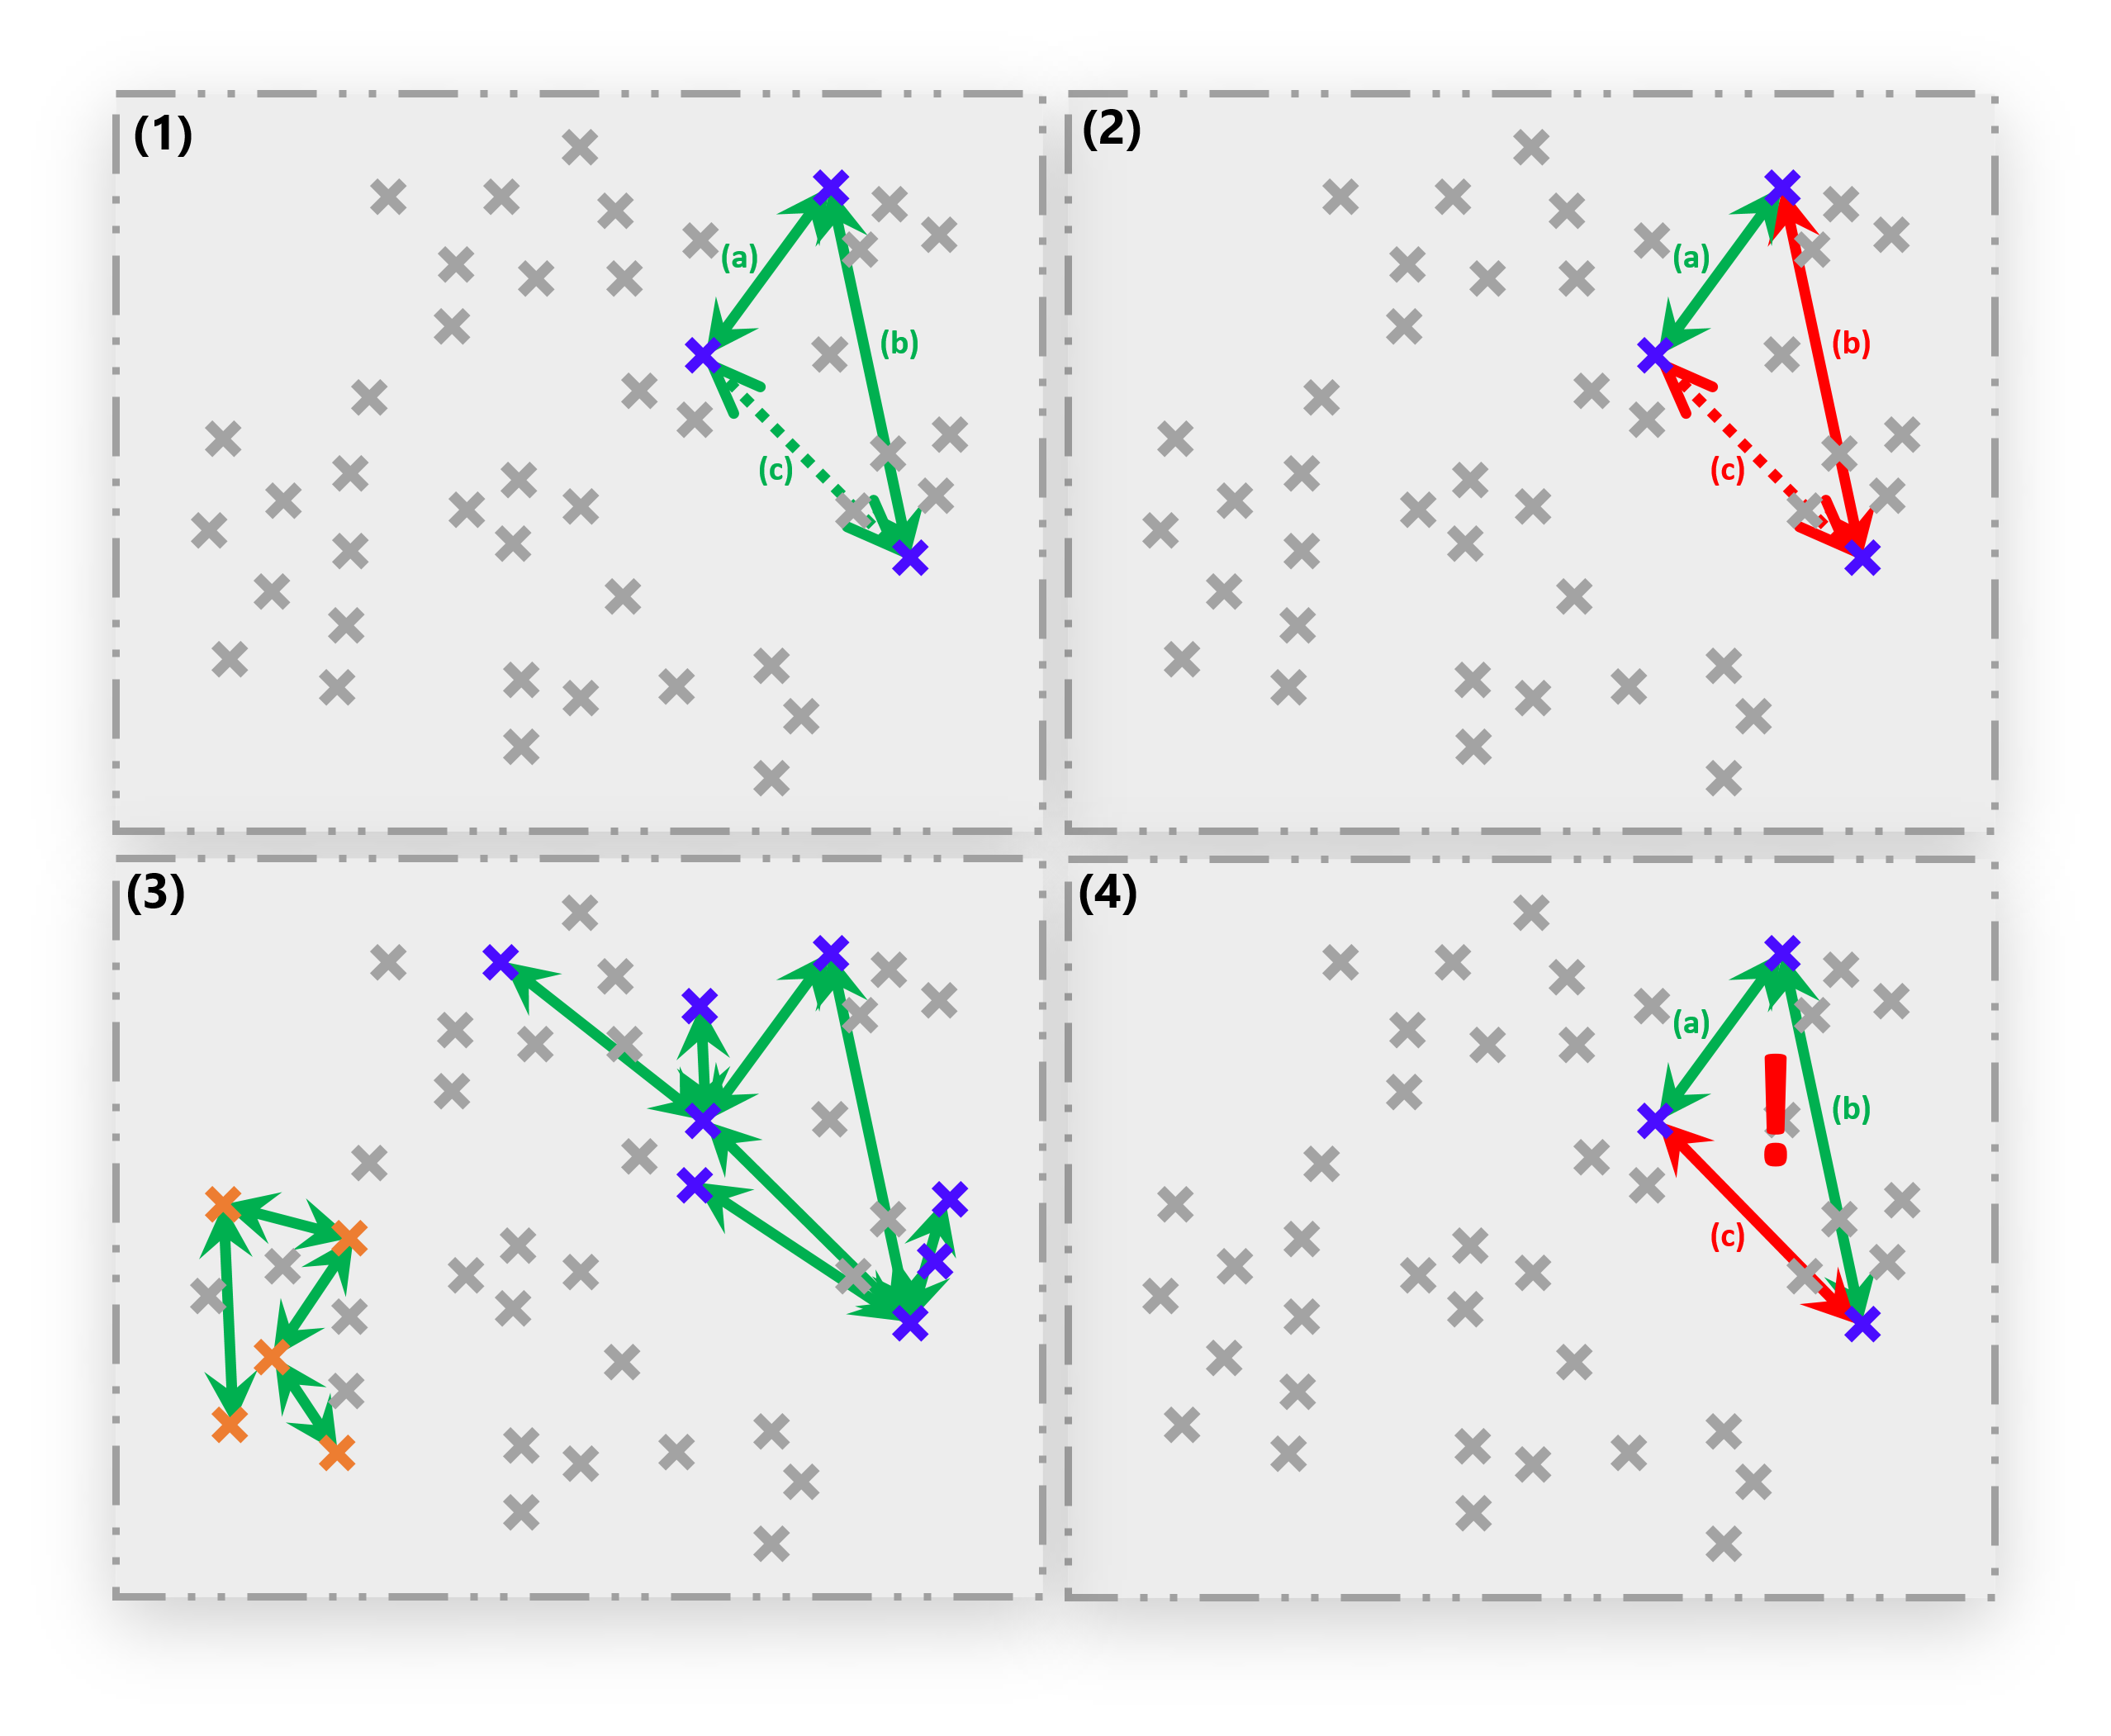
\includegraphics[width=0.70\textwidth]{figures/example-constraints-transitivity}
		\caption{
			Exemples des propriétés de transitivité des contraintes \texttt{MUST-LINK} (flèches vertes) et \texttt{CANNOT-LINK} (flèches rouges). \textbf{(1)} et \textbf{(2)} représentent les possibilités de déduction d'une contrainte (\texttt{(c)}) en fonction des deux autres (\texttt{(a)} et \texttt{(b)}). \textbf{(3)} représente deux composants connexes définis par la transitivité des contraintes \texttt{MUST-LINK}. Enfin, \textbf{(4)} représente un cas de conflit où une contrainte (\texttt{(c)}) ne correspond pas à sa déduction faite à partir des autres contraintes (\texttt{(a)} et \texttt{(b)}).
		}
		\label{figure:C.1.2-DESCRIPTION-IMPLEMENTATION-INTERACTIVE-CLUSTERING-CONTRAINTES-TRANSITIVITE}
	\end{figure}
	
	% cognitivefactory.interactive-clustering.constraints : Exemple.
	Un exemple d'utilisation du module de gestion de contraintes est consultable dans \textsc{Code~\ref{code:C.1.2-DESCRIPTION-IMPLEMENTATION-INTERACTIVE-CLUSTERING-GESTION-CONTRAINTES}}.
	
	\begin{lstlisting}[
		language=Python,
		caption={Démonstration de notre implémentation de gestion des contraintes sur le jeu d'exemples.},
		label={code:C.1.2-DESCRIPTION-IMPLEMENTATION-INTERACTIVE-CLUSTERING-GESTION-CONTRAINTES},
	]
# Import des dépendances.
from cognitivefactory.interactive_clustering.constraints.factory import managing_factory

# Création du gestionnaire de contraintes.
constraints_manager = managing_factory(
	manager="binary",
	list_of_data_IDs = list(dict_of_texts.keys()),
	# ["0", "1", "2", "3", "4", "5", ..., "N"]
)

# Ajout de contraintes.
constraints_manager.add_constraint(
	data_ID1="0",  # "Comment signaler un vol de carte bancaire ?"
	data_ID2="1",  # "J'ai égaré ma carte bancaire, que faire ?"
	constraint_type="MUST_LINK",
)
constraints_manager.add_constraint(
	data_ID1="3",  # "Le distributeur a avalé ma carte !"
	data_ID2="4",  # "En retirant de l'argent, le GAB a gardé ma carte..."
	constraint_type="MUST_LINK",
)
constraints_manager.add_constraint(
	data_ID1="0",  # "Comment signaler un vol de carte bancaire ?"
	data_ID2="N",  # "Pourquoi le sans contact ne fonctionne pas ?"
	constraint_type="CANNOT_LINK",
)
# NB: ajouter une contrainte "MUST_LINK" entre "1" et "N" lèverait une erreur.

# Récupération des composants connexes.
connected_components = constraints_manager.get_connected_components()
"""
[['0', '1'],
 ['2'],
 ['3', '4'],
 ['5'],
 ['N']]
"""
	\end{lstlisting}
	
	
	%%%
	%%% Subsection C.1.3: Algorithme de \textit{clustering} sous contraintes.
	%%%
	\subsection{Algorithme de \textit{clustering} sous contraintes}
	\label{annex:C.1.3-DESCRIPTION-IMPLEMENTATION-INTERACTIVE-CLUSTERING-ALGORITHMES-CLUSTERING-SOUS-CONTRAINTES}
	
	% cognitivefactory.interactive-clustering.clustering
	En ce qui concerne le \textbf{regroupement automatique} des données par similarité, nous utilisons le module \texttt{clustering} \footnote{
		\url{https://cognitivefactory.github.io/interactive-clustering/reference/cognitivefactory/interactive_clustering/clustering/}
	} de la librairie \texttt{cognitivefactory-interactive-clustering}.
	
	% cognitivefactory.interactive-clustering.utils.clustering : Implémentation.
	Ce module met à disposition cinq algorithmes de \textit{clustering} sous contraintes :
	\begin{enumerate}
		\item \textbf{\texttt{KMeans}}, dans sa version \texttt{COP-KMeans} (\cite{wagstaff-etal:2001:constrained-kmeans-clustering}), noté \texttt{clust.kmeans.cop}, et sa version \texttt{MPC-KMeans} (\cite{khan-etal:2012:multiple-parameter-based}), noté \texttt{clust.kmeans.mpc}) ;
		\item \textbf{\texttt{DBscan}}, dans sa version \texttt{C-DBScan} (\cite{ruiz-etal:2010:densitybased-semisupervised-clustering}), noté \texttt{clust.cdbscan} ;
		\item \textbf{Hiérarchique} (\cite{davidson-ravi:2005:agglomerative-hierarchical-clustering}), avec quatre métriques de distances : \texttt{single} (noté \texttt{clust.hier.sing}), \texttt{complete} (noté \texttt{clust.hier.comp}), \texttt{average} (noté \texttt{clust.hier.avg}) et \texttt{ward} (noté \texttt{clust.hier.ward}) ;
		\item \textbf{Spectral}, dans sa version \texttt{SPEC} (\cite{kamvar-etal:2003:spectral-learning}), noté \texttt{clust.spec} ;
		\item \textbf{Propagation par affinité} (\cite{givoni-frey:2009:semisupervised-affinity-propagation}), noté \texttt{clust.affprop}.
	\end{enumerate}
	
	Une classe abstraite définit les prérequis des algorithmes implémentés (avoir une méthode \texttt{cluster}) et une \textit{factory} est disponible pour instancier rapidement un objet de \textit{clustering}.
	% cognitivefactory.interactive-clustering.clustering : Exemple.
	Enfin, un exemple d'utilisation de ce module est consultable dans \textsc{Code~\ref{code:C.1.3-DESCRIPTION-IMPLEMENTATION-INTERACTIVE-CLUSTERING-CLUSTERING}}.
	
	
	\begin{lstlisting}[
		language=Python,
		caption={Démonstration de notre implémentation du \textit{clustering} sous contraintes sur le jeu d'exemples.},
		label={code:C.1.3-DESCRIPTION-IMPLEMENTATION-INTERACTIVE-CLUSTERING-CLUSTERING},
	]
# Import des dépendances.
from cognitivefactory.interactive_clustering.clustering.factory import clustering_factory

# Initialiser un objet de clustering.
clustering_model = clustering_factory(
	algorithm="kmeans",
	model="COP",
	random_seed=42,
)

# Lancer le clustering.
clustering_result = clustering_model.cluster(
	constraints_manager=constraints_manager,
	nb_clusters=2,
	vectors=dict_of_vectors,
)
"""
{"0": 0,  # "Comment signaler un vol de carte bancaire ?"
 "1": 0,  # "J'ai égaré ma carte bancaire, que faire ?"
 "2": 0,  # "J'ai perdu ma carte de paiement"
 "3": 1,  # "Le distributeur a avalé ma carte !"
 "4": 1,  # "En retirant de l'argent, le GAB a gardé ma carte..."
 "5": 1,  # "Le distributeur ne m'a pas rendu ma carte bleue."
 # ...
 "N": 1}  # "Pourquoi le sans contact ne fonctionne pas ?"
"""
	\end{lstlisting}
	
	% cognitivefactory.interactive-clustering.utils.clustering : Historique.
	\begin{leftBarInformation}
		Dans le cadre d'un projet étudiant avec l'École d'Ingénieurs Télécom Physique Strasbourg (au cours de l'année 2022), les implémentations des algorithmes \texttt{MPC-KMeans}, \texttt{C-DBScan} et de propagation par affinité ont été ajoutées. Les élèves ont conclu ce projet d'extension en suggérant de se concentrer sur l'étude du C-DBScan car les deux autres algorithmes étaient soit trop instables, soit trop gourmand en temps de calcul.
		Les autres algorithmes (\texttt{COP-KMeans}, hiérarchique et spectral) ont été implémentés au début de ce doctorat.
	\end{leftBarInformation}
	
	
	%%%
	%%% Subsection C.1.4: Algorithme d'échantillonnage de contraintes.
	%%%
	\subsection{Algorithme d'échantillonnage de contraintes}
	\label{annex:C.1.4-DESCRIPTION-IMPLEMENTATION-INTERACTIVE-CLUSTERING-ALGORITHMES-ECHANTILLONNAGE-DE-CONTRAINTES}
	
	% cognitivefactory.interactive-clustering.sampling
	En ce qui concerne l'\textbf{échantillonnage} de contraintes à annoter, nous utilisons le module \texttt{sampling} \footnote{
		\url{https://cognitivefactory.github.io/interactive-clustering/reference/cognitivefactory/interactive_clustering/sampling/}
	} de la librairie \texttt{cognitivefactory-interactive-clustering}.
	
	% cognitivefactory.interactive-clustering.utils.sampling : Implémentation.
	Cet échantillonnage correspond à la sélection de couple de données.
	Par défaut, l'échantillonnage est purement aléatoire.
	Cependant, plusieurs options sont disponibles :
	
	\begin{itemize}
		\item[\(\bullet\)] une restriction sur la \textit{distance} pouvant imposer aux données d'être les plus proches ou les plus éloignées du corpus ;
		\item[\(\bullet\)] une restriction sur le \textit{résultat du clustering} pouvant imposer aux données d'être issues d'un même \textit{cluster} ou de \textit{clusters} différents,
		\item[\(\bullet\)] une restriction pour exclure les contraintes \textit{déjà annotées},
		\item[\(\bullet\)] et enfin une restriction pour exclure les contraintes \textit{déjà déduites} par transitivité.
	\end{itemize}
	
	% cognitivefactory.interactive-clustering.utils.sampling : Par défaut.
	Sur cette base, nous définissons quatre niveaux d'échantillonnage facilement identifiables pour nos études :
	\begin{enumerate}
		\item Un échantillonnage \textbf{purement aléatoire}, en excluant toutes les contraintes déjà annotées ou déduites, noté \texttt{samp.random.full} ;
		\item Un échantillonnage \textbf{pseudo-aléatoire} de données issues d'un \textbf{même \textit{cluster}}, en excluant toutes les contraintes déjà annotées ou déduites, noté \texttt{samp.random.same} ;
		\item Un échantillonnage des données issues d'un \textbf{même \textit{cluster}} et étant \textbf{les plus éloignées} les unes des autres, noté \texttt{samp.farhtest.same} (cf. \textsc{Figure~\ref{figure:C.1.4-DESCRIPTION-IMPLEMENTATION-INTERACTIVE-CLUSTERING-CONTRAINTES-SAMPLING}}) ;
		\item Un échantillonnage des données issues de \textbf{\textit{clusters} différents} et étant \textbf{les plus proches} les unes des autres, noté \texttt{samp.closest.diff} (cf. \textsc{Figure~\ref{figure:C.1.4-DESCRIPTION-IMPLEMENTATION-INTERACTIVE-CLUSTERING-CONTRAINTES-SAMPLING}}).
	\end{enumerate}
	
	\begin{figure}[!htb]
		\centering
		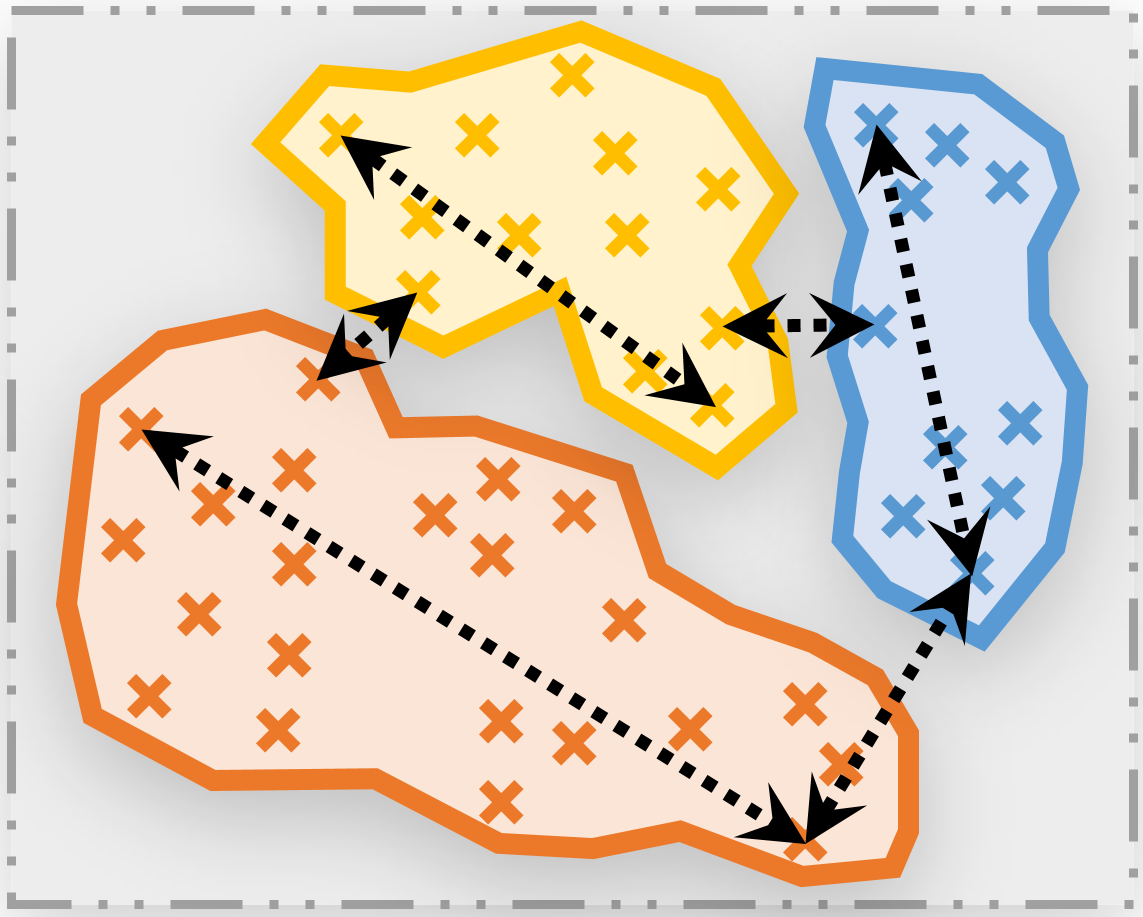
\includegraphics[width=0.35\textwidth]{figures/example-sampling}
		\caption{
			Exemples d'échantillonnages, sur la base de trois clusters, de données issues de mêmes \textit{clusters} et étant les plus éloignées les unes des autres (\texttt{samp.farhtest.same}), et de données issues de clusters différents et étant les plus proches les unes des autres (\texttt{samp.closest.diff}).
		}
		\label{figure:C.1.4-DESCRIPTION-IMPLEMENTATION-INTERACTIVE-CLUSTERING-CONTRAINTES-SAMPLING}
	\end{figure}

	Une classe abstraite définit les prérequis des algorithmes implémentés (avoir une méthode \texttt{sample}) et une \textit{factory} est disponible pour instancier rapidement un objet d'échantillonnage.
	% cognitivefactory.interactive-clustering.sampling : Exemple.
	Un exemple d'utilisation de ce module est consultable dans \textsc{Code~\ref{code:C.1.4-DESCRIPTION-IMPLEMENTATION-INTERACTIVE-CLUSTERING-SAMPLING}}.
	
	\begin{lstlisting}[
		language=Python,
		caption={Démonstration de notre implémentation de l'échantillonnage sur le jeu d'exemples.},
		label={code:C.1.4-DESCRIPTION-IMPLEMENTATION-INTERACTIVE-CLUSTERING-SAMPLING},
	]
# Import des dépendances.
from cognitivefactory.interactive_clustering.sampling.factory import sampling_factory

# Initialiser un objet d'échantillonnage.
sampler = sampling_factory(
	algorithm="random",
	random_seed=42,
)

# Run sampling.
selection = sampler.sample(
	constraints_manager=constraints_manager,
	nb_to_select=2,
	clustering_result=clustering_result,  # optionnel
	vectors=dict_of_vectors,  # optionnel
)
"""
[("0", '5"),  # "Comment signaler un vol de carte bancaire ?" vs "Le distributeur ne m'a pas rendu ma carte bleue."
 ("0", '2"),  # "Comment signaler un vol de carte bancaire ?" vs "J'ai perdu ma carte de paiement"
 ("2", 'N")]  # "J'ai perdu ma carte de paiement" vs "Pourquoi le sans contact ne fonctionne pas ?"
"""
	\end{lstlisting}
	
	
	%%%%%--------------------------------------------------------------------
	%%%%% Section C.2: Implémentation de la librairie \texttt{cognitivefactory-interactive-clustering}
	%%%%%--------------------------------------------------------------------
	%\newpage
	\section{Implémentation de la librairie \\ \texttt{cognitivefactory-features-maximization-metric}}
\label{annex:C.2-DESCRIPTION-IMPLEMENTATION-FEATURES-MAXIMIZATION-METRIC}
	
	% Généralités.
	La librairie \texttt{cognitivefactory-features-maximization-metric} (\cite{schild:2023:cognitivefactory-featuresmaximizationmetric}) ...
	\todo[inline]{introduction à rédiger}
	
	% Information : comme y accéder.
	\begin{leftBarInformation}
		La documentation technique est accessible au lien suivant : \url{https://cognitivefactory.github.io/features-maximization-metric/}.
	\end{leftBarInformation}
	
	
	%%%%%--------------------------------------------------------------------
	%%%%% Section C.3: Implémentation de la librairie \texttt{cognitivefactory-interactive-clustering}
	%%%%%--------------------------------------------------------------------
	%\newpage
	\section{Implémentation de l'application web \texttt{cognitivefactory-interactive-clustering-gui}}
\label{section:C.3-DESCRIPTION-IMPLEMENTATION-INTERACTIVE-CLUSTERING-GUI}

	% INTRODUCTION DE L'ANNEXE.
	Au cours de ce doctorat, nous avons implémenté notre méthodologie de \textit{clustering} interactif au sein d'une application web.
	Celle-ci dispose de plusieurs fonctionnalités telles que :
	\begin{itemize}
		\item la gestion du projet, de ses données et de ses paramétrages ;
		\item la gestion et l'annotation de contraintes, ainsi que la vérification des propriétés de transitivités ;
		\item la gestion des étapes d'une itération de la méthode ;
		\item l'exécution asynchrone des divers algorithmes de la méthode (prétraitement, vectorisation, clustering, échantillonnage) ;
		\item quelques scripts d'analyses.
			% \footnote{Les scripts d'analyses concernent la visualisation des clusters et des composants connexes au cours des itérations, la vérification de la pertinence avec l'analyse des patterns linguistiques et les résumés automatiques de thématique, et l'analyse de la rentabilité avec l'évolution de la similarité entre résultats de \textit{clustering}.}.
	\end{itemize}
	
	Nous présenterons succinctement cette application ci-dessous à l'aide de captures d'écrans.
	
	% Information : comme y accéder.
	\begin{leftBarInformation}
		L'application est accessible dans \cite{schild-etal:2022:cognitivefactory-interactiveclusteringgui}.
		La documentation technique est accessible au lien suivant : \url{https://cognitivefactory.github.io/interactive-clustering-gui/}.
	\end{leftBarInformation}
	
	% Note de l'auteur : en cours de maintenance.
	\begin{leftBarAuthorOpinion}
		Suite aux diverses études menées au cours de ce doctorat, certaines pages sont en cours de refonte, notamment les pages d'analyses (suite aux conclusions des \textsc{Section~\ref{section:4.4-HYPOTHESE-PERTINENCE}} et \textsc{Section~\ref{section:4.5-HYPOTHESE-RENTABILITE}}) et les pages de documentations (suite à discussion en \textsc{Chapitre~\ref{chapter:5-GUIDE}}.
	\end{leftBarAuthorOpinion}
	
	
	%%% Page d'accueil de l'application
	\newpage
	\paragraph{Page d'accueil de l'application (\textsc{Figure~\ref{figure:C-WEB-APPLICATION-ACCUEIL}}) :}
		C'est la page de bienvenu de l'application.
		Nous y trouvons une description rapide de la méthode ainsi qu'une liste des questions fréquentes à son sujet.
		Le bouton en haut à gauche permettra toujours de revenir sur cette page.
		
		% Capture d'écran: Page d'accueil de l'application.
		\begin{figure}[H]
			\centering
			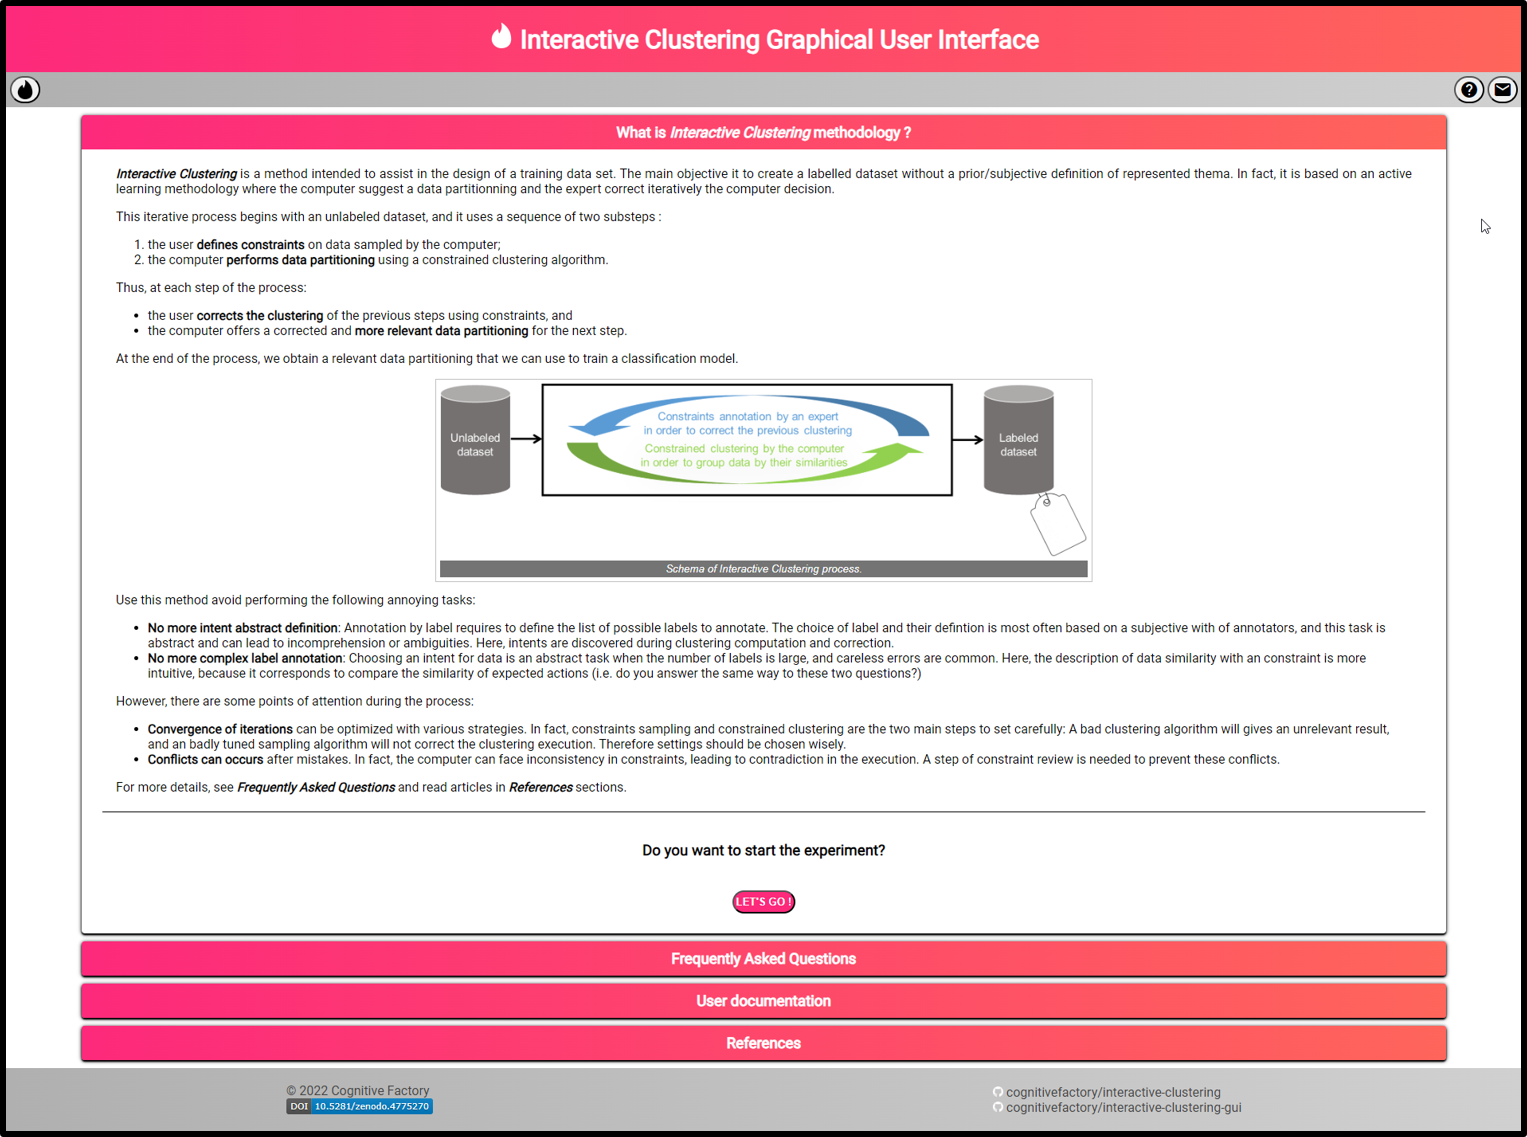
\includegraphics[width=0.95\textwidth]{figures/interactive-clustering-application-accueil-application}
			\caption{
				Capture d'écran de l'application web implémentant notre méthodologie de \textit{clustering} interactif : \textbf{page d'accueil de l'application}.
			}
			\label{figure:C-WEB-APPLICATION-ACCUEIL}
		\end{figure}
	
	
	%%% Page de gestion des projets
	\newpage
	\paragraph{Page de gestion des projets (\textsc{Figure~\ref{figure:C-WEB-APPLICATION-LISTE-PROJETS}}) :}
		Cette page liste les projets existants sous la forme de tuiles contenant les informations importantes : nom, date de création, nombre d'itérations de la méthode, et statut du projet (nous y reviendrons plus tard).
		Il est possible de télécharger un projet au format \texttt{.zip} ou de le supprimer.
		Pour créer un projet, le bouton \texttt{ADD NEW} ouvre un petit formulaire demandant le nom du projet et la liste des textes à annoter (au format \texttt{.csv} séparateur '\texttt{;}').
		Il est aussi possible d'importer un projet à l'aide d'une archive \texttt{.zip} téléchargée au préalable.
		Le bouton \texttt{LOAD} mène à la page d'accueil du projet sélectionné.
		
		% Capture d'écran: liste des projets.
		\begin{figure}[H]
			\centering
			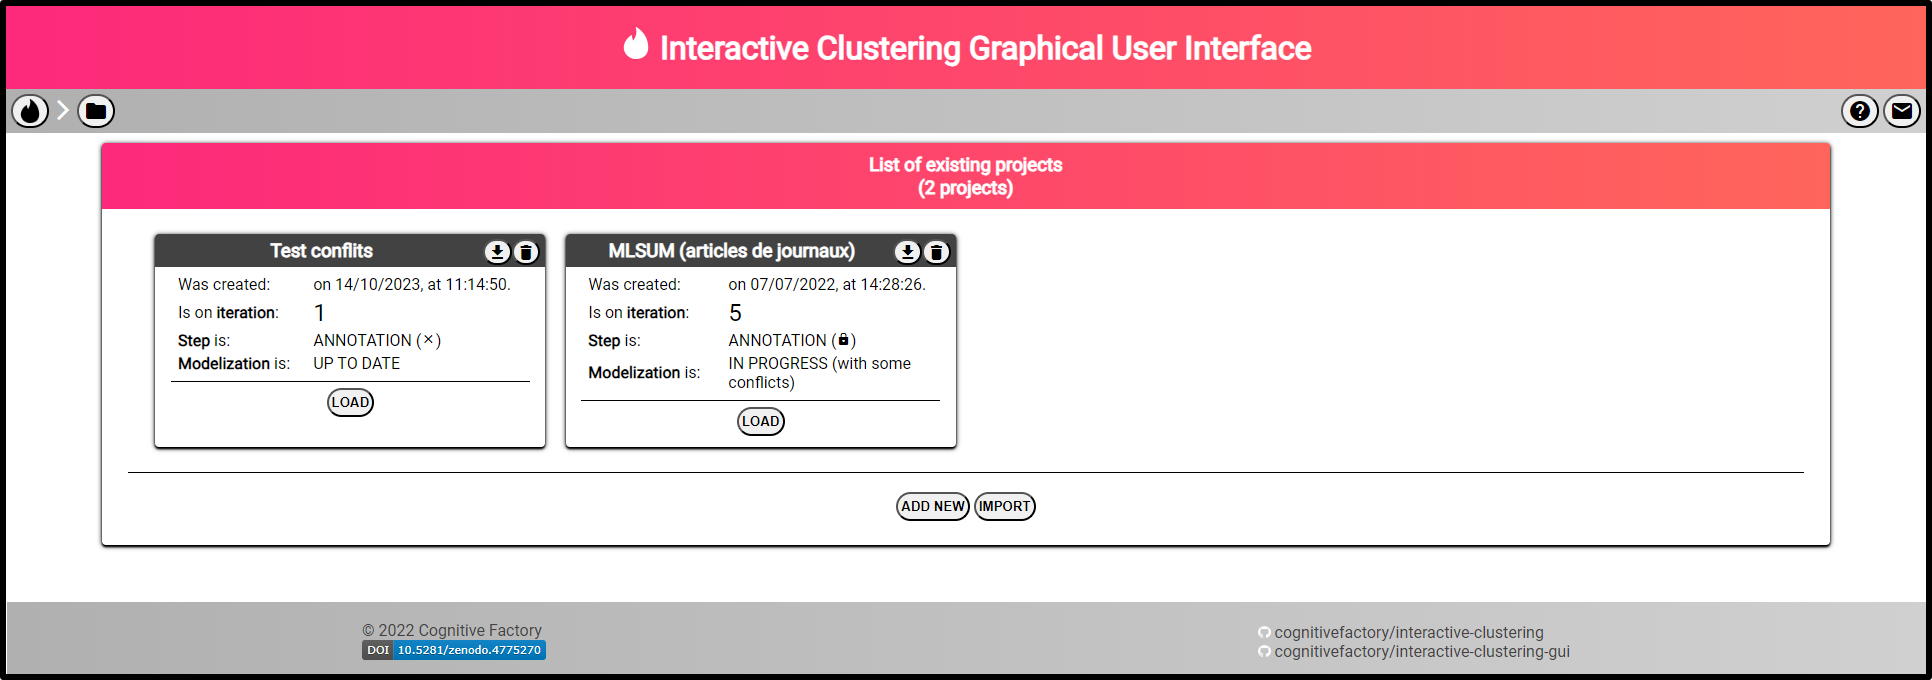
\includegraphics[width=0.95\textwidth]{figures/interactive-clustering-application-liste-projets}
			\caption{
				Capture d'écran de l'application web implémentant notre méthodologie de \textit{clustering} interactif : \textbf{page de gestion des projets}.
			}
			\label{figure:C-WEB-APPLICATION-LISTE-PROJETS}
		\end{figure}
	
	
	%%% Page d'accueil du projet en cours
	\newpage
	\paragraph{Page d'accueil du projet en cours (\textsc{Figure~\ref{figure:C-WEB-APPLICATION-ACCUEIL-PROJET}}) :}
		\todo[inline]{à rédiger}
	
		% Capture d'écran: accueil projet.
		\begin{figure}[H]
			\centering
			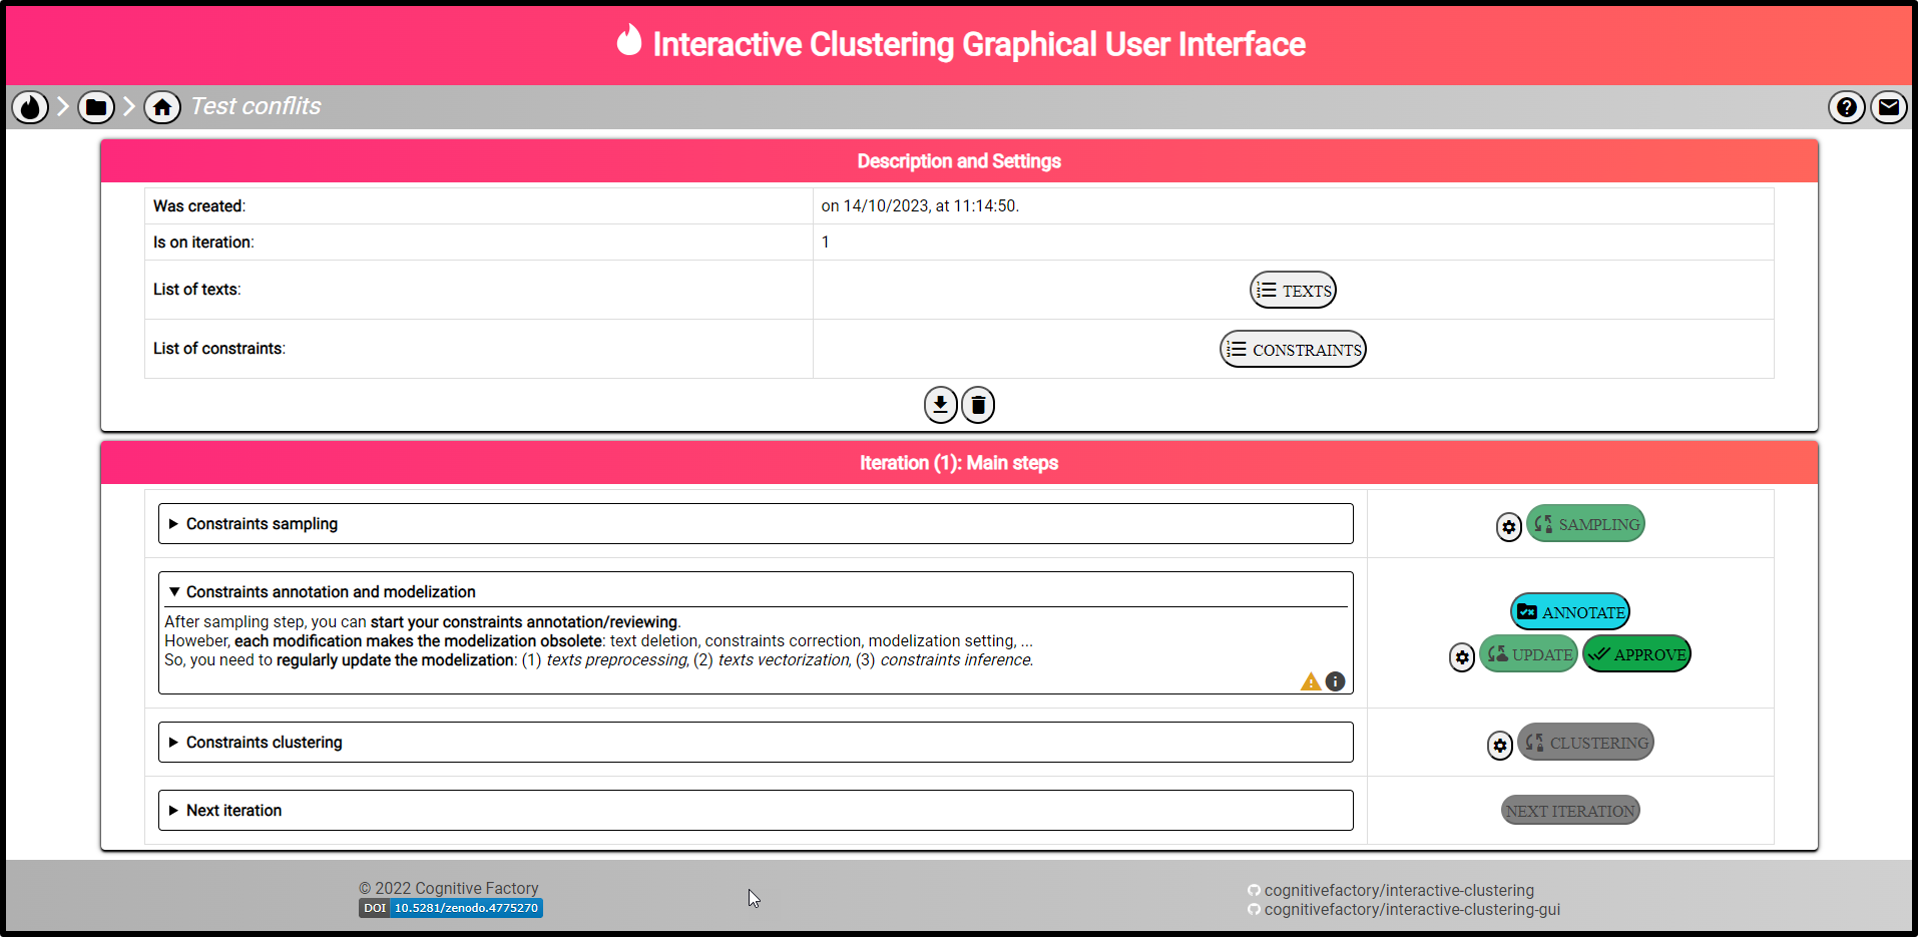
\includegraphics[width=0.95\textwidth]{figures/interactive-clustering-application-accueil-projet}
			\caption{
				Capture d'écran de l'application web implémentant notre méthodologie de \textit{clustering} interactif : \textbf{page d'accueil du projet en cours}.
			}
			\label{figure:C-WEB-APPLICATION-ACCUEIL-PROJET}
		\end{figure}
	
	
	%%% Diagramme d'états de l'application et gestion des exécutions asynchrones
	\newpage
	\paragraph{Diagramme d'états de l'application et gestion des exécutions asynchrones (\textsc{Figure~\ref{figure:C-WEB-APPLICATION-DIAGRAMME-ETATS}}) :}
		\todo[inline]{à rédiger}
	
		% Capture d'écran: accueil projet.
		\begin{figure}[H]
			\centering
			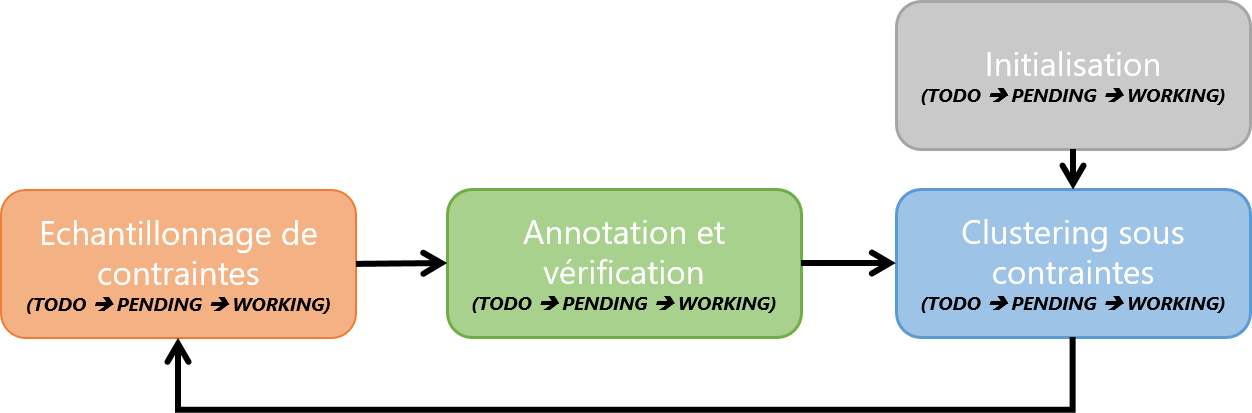
\includegraphics[width=0.95\textwidth]{figures/interactive-clustering-application-diagramme-etats}
			\caption{
				\textbf{Diagramme d'états} simplifié de l'application web implémentant notre méthodologie de \textit{clustering} interactif.
			}
			\label{figure:C-WEB-APPLICATION-DIAGRAMME-ETATS}
		\end{figure}
	
	
	%%% Page de gestion des paramètres
	\newpage
	\paragraph{Page de gestion des paramètres (\textsc{Figure~\ref{figure:C-WEB-APPLICATION-PARAMETRAGE}}) :}
		\todo[inline]{à rédiger}
	
		% Capture d'écran: gestion des paramètrages.
		\begin{figure}[H]
			\centering
			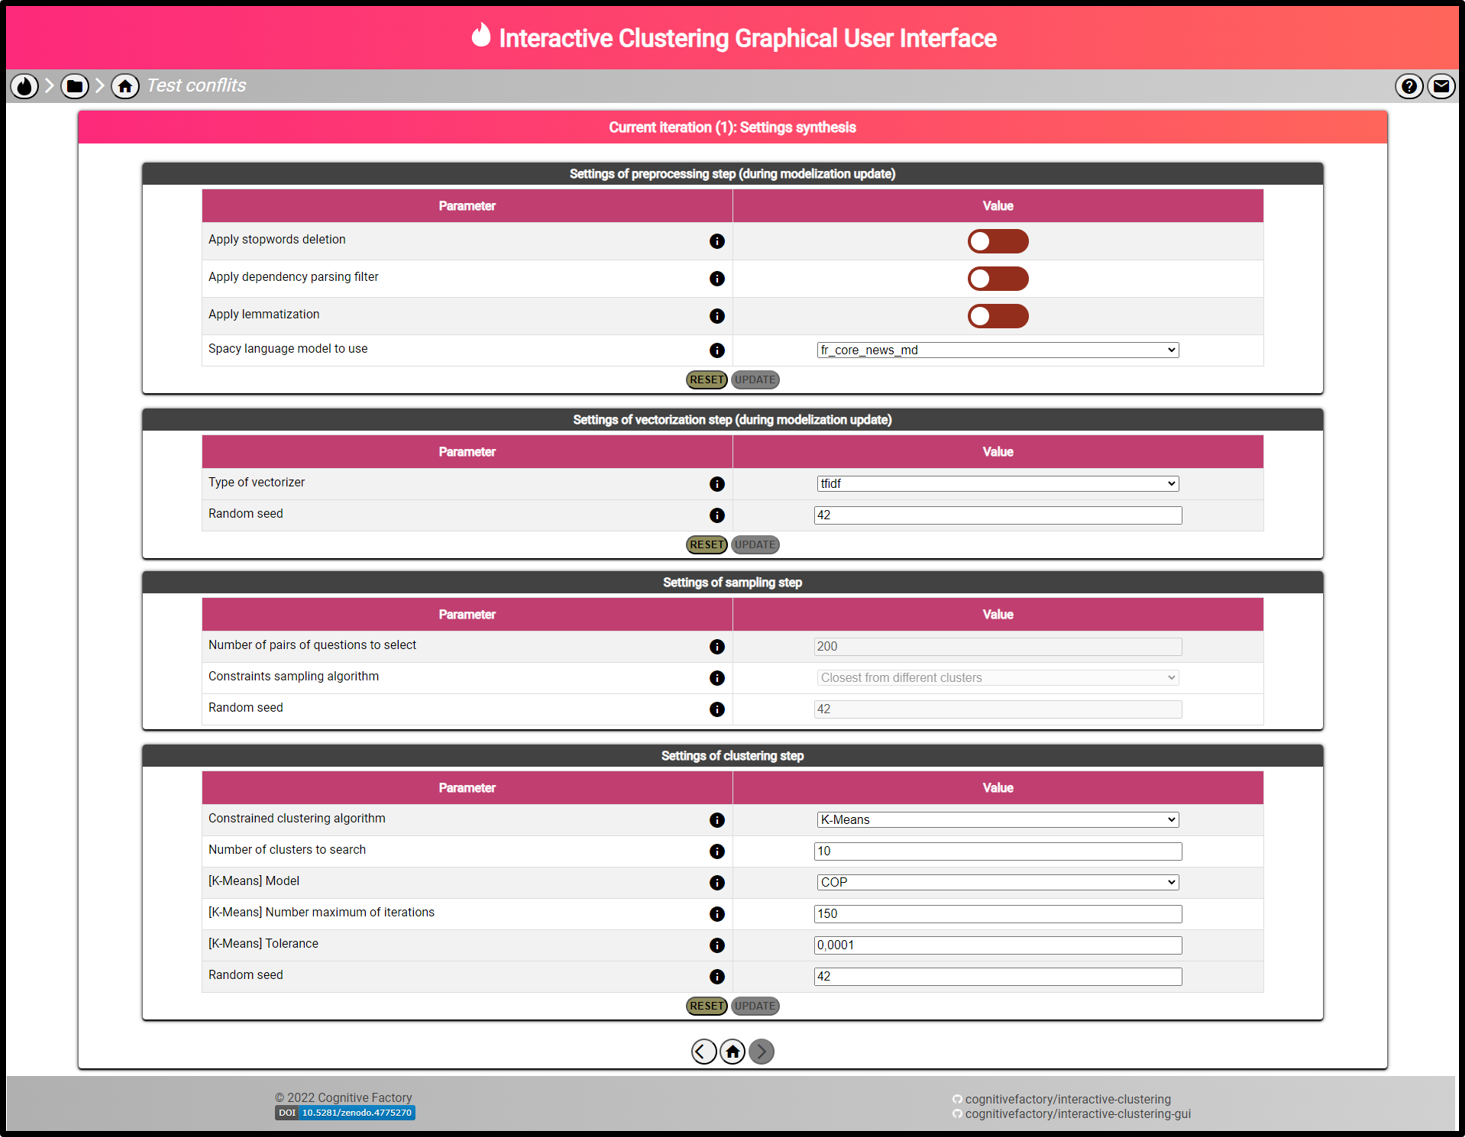
\includegraphics[width=0.95\textwidth]{figures/interactive-clustering-application-parametres}
			\caption{
				Capture d'écran de l'application web implémentant notre méthodologie de \textit{clustering} interactif : \textbf{page de gestion des paramètres}.
			}
			\label{figure:C-WEB-APPLICATION-PARAMETRAGE}
		\end{figure}
	
	
	%%% Page d'inventaire des textes
	\newpage
	\paragraph{Page d'inventaire des textes (\textsc{Figure~\ref{figure:C-WEB-APPLICATION-INVENTAIRE-TEXTES}}) :}
		\todo[inline]{à rédiger}
	
		% Capture d'écran: inventaire des textes.
		\begin{figure}[H]
			\centering
			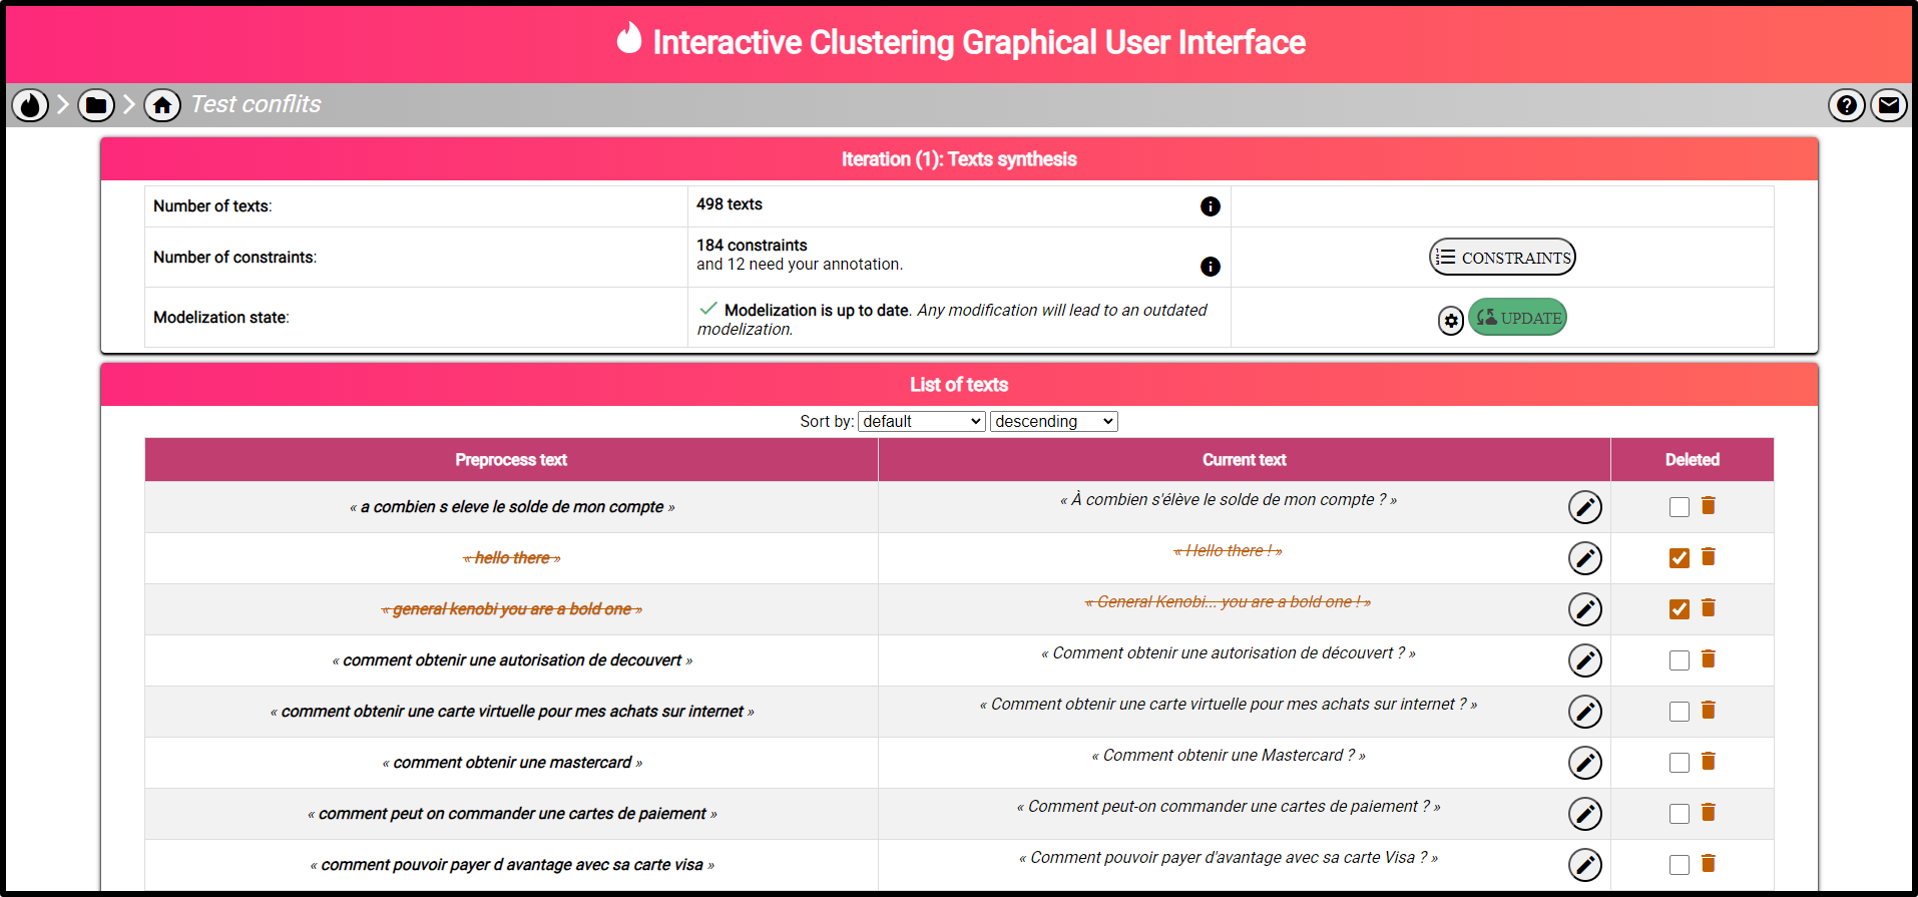
\includegraphics[width=0.95\textwidth]{figures/interactive-clustering-application-textes}
			\caption{
				Capture d'écran de l'application web implémentant notre méthodologie de \textit{clustering} interactif : \textbf{page d'inventaire des textes}.
			}
			\label{figure:C-WEB-APPLICATION-INVENTAIRE-TEXTES}
		\end{figure}
	
	
	%%% Page d'inventaire des contraintes
	\newpage
	\paragraph{Page d'inventaire des contraintes (\textsc{Figure~\ref{figure:C-WEB-APPLICATION-INVENTAIRE-CONTRAINTES}}) :}
		\todo[inline]{à rédiger}
	
		% Capture d'écran: inventaire des contraintes.
		\begin{figure}[H]
			\centering
			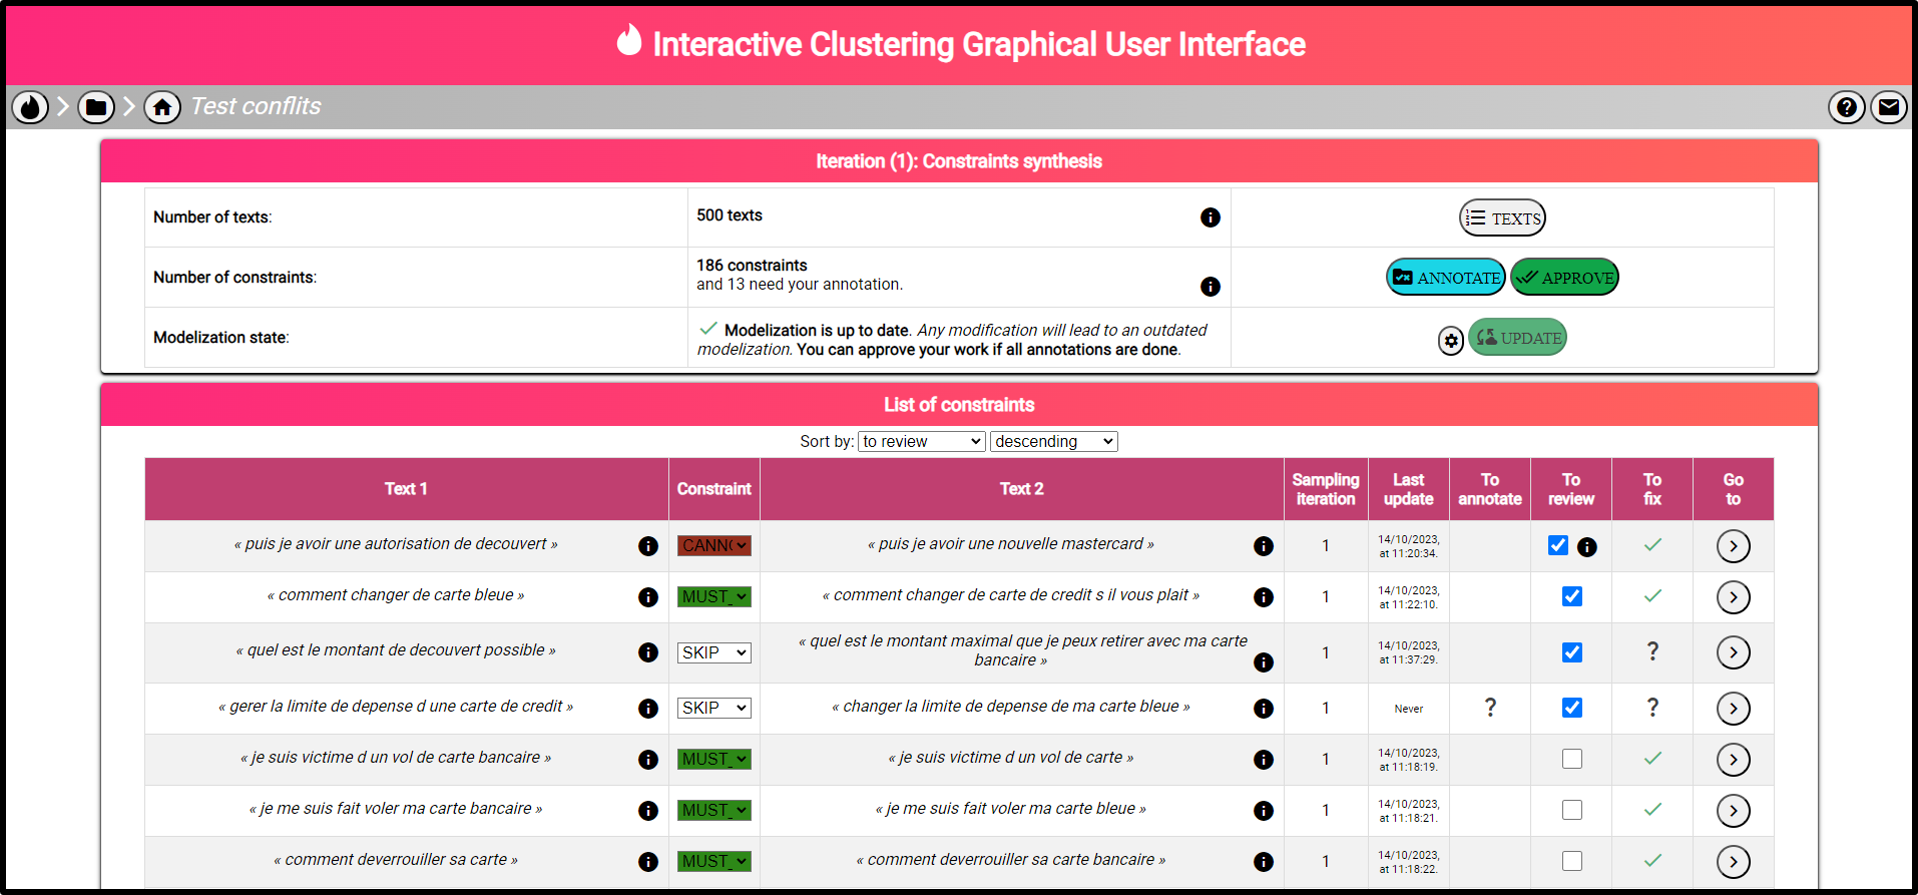
\includegraphics[width=0.95\textwidth]{figures/interactive-clustering-application-contraintes}
			\caption{
				Capture d'écran de l'application web implémentant notre méthodologie de \textit{clustering} interactif : \textbf{page d'inventaire des contraintes}.
			}
			\label{figure:C-WEB-APPLICATION-INVENTAIRE-CONTRAINTES}
		\end{figure}
	
	
	%%% Page d'annotation d'une contrainte
	\newpage
	\paragraph{Page d'annotation d'une contrainte (\textsc{Figure~\ref{figure:C-WEB-APPLICATION-ANNOTATION}} et \textsc{Figure~\ref{figure:C-WEB-APPLICATION-CONFLIT}}) :}
		\todo[inline]{à rédiger}
	
		% Capture d'écran: annotation.
		\begin{figure}[H]
			\centering
			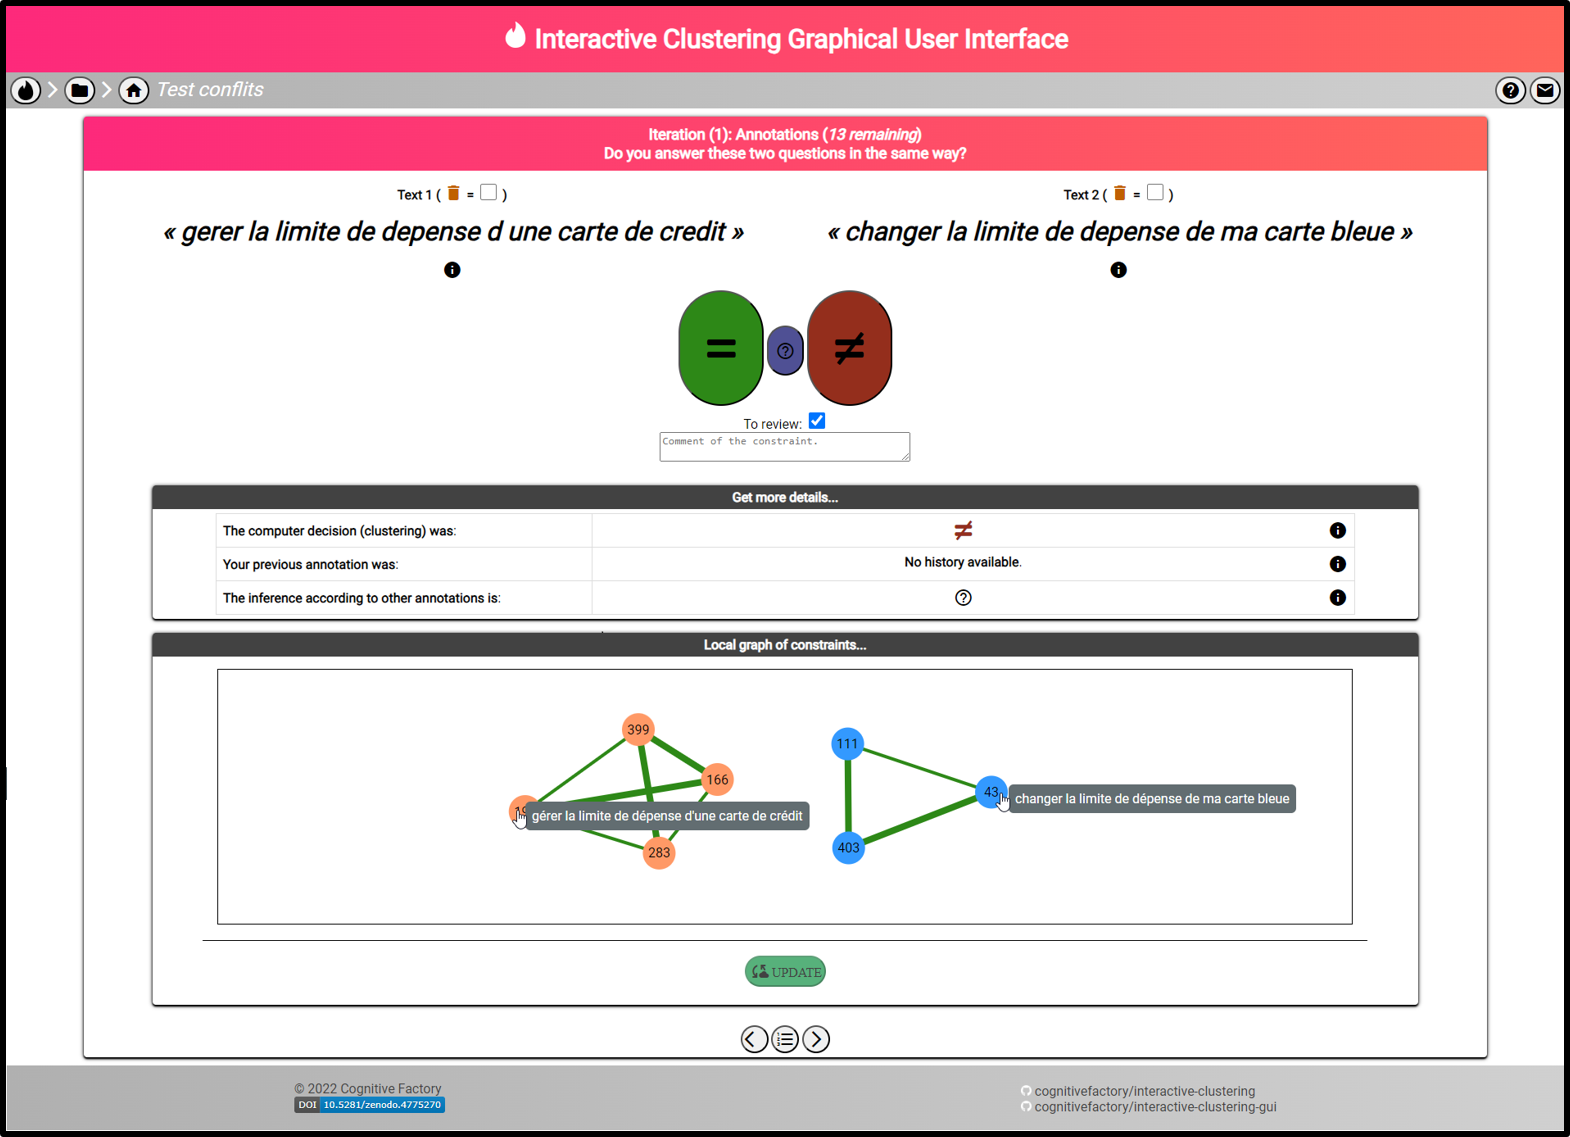
\includegraphics[width=0.95\textwidth]{figures/interactive-clustering-application-annotation-0full}
			\caption{
				Capture d'écran de l'application web implémentant notre méthodologie de \textit{clustering} interactif : \textbf{page d'annotation d'une contrainte}.
			}
			\label{figure:C-WEB-APPLICATION-ANNOTATION}
		\end{figure}
		
		% Capture d'écran: conflit d'annotation.
		\begin{figure}[H]
			\centering
			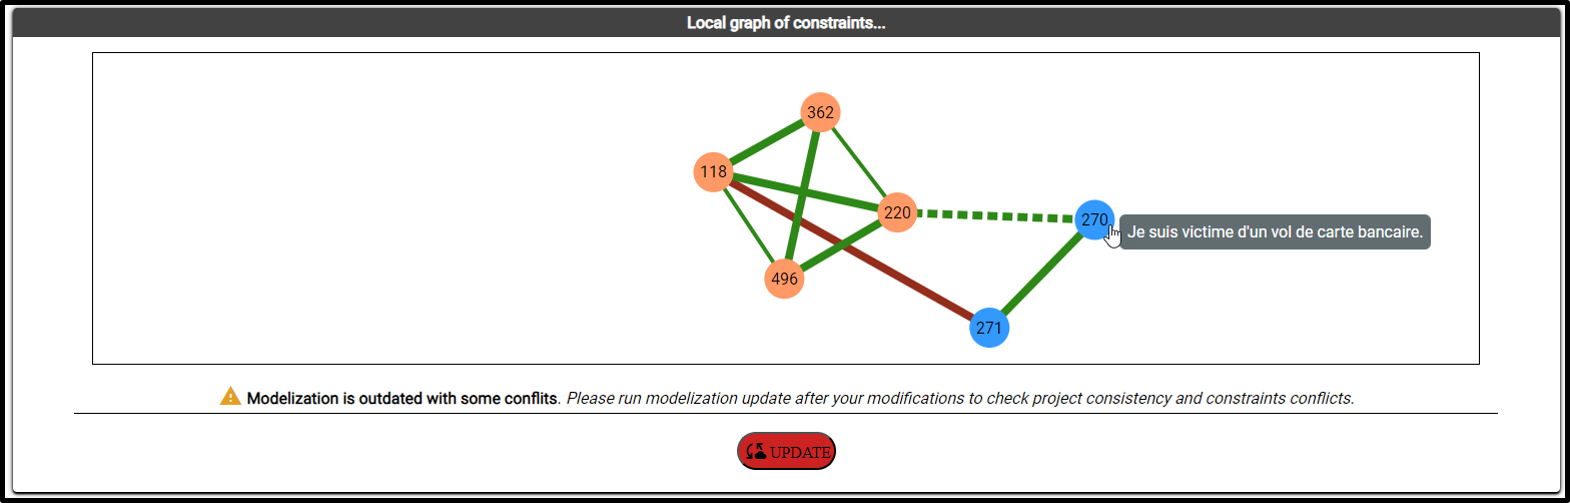
\includegraphics[width=0.95\textwidth]{figures/interactive-clustering-application-annotation-4conflit}
			\caption{
				Capture d'écran de l'application web implémentant notre méthodologie de \textit{clustering} interactif : \textbf{graphe de contraintes présentant un conflit d'annotation}.
			}
			\label{figure:C-WEB-APPLICATION-CONFLIT}
		\end{figure}